 \chapter{The Multiscale and Signed Frangi Filter} \label{ch:multifrangi}
    
    
    	\begin{figure}[p] \centering % scale sweep, large plate
    	\subfloat{        \label{fig:scalesweep-1p}\includegraphics[width=\linewidth]{{{scalesweep_stitch_BN2315363_plate}}}
    	} \\[-0.5cm]
    	\subfloat{        \label{fig:scalesweep-1i}\includegraphics[width=\linewidth]{{{scalesweep_stitch_BN2315363_inset}}}
    	} \\[-0.5cm]
    	\subfloat{        
    		\label{fig:scalesweep-1c}\includegraphics[width=.75\linewidth]{{{scalesweep_colorbar}}}
    	} \\
    	% should i use the real sample names? or obfuscate?
    	\caption{Example scalewise Frangi output (plate and inset) (Example 1)}
    	\label{fig:scalesweep-1}
    \end{figure}
    
    \begin{figure}[p] \centering % scale sweep, small plate
    	\subfloat{        \label{fig:scalesweep-2p}\includegraphics[width=\linewidth]{{{scalesweep_stitch_BN5280796_plate}}}
    	} \\[-0.5cm]
    	\subfloat{        \label{fig:scalesweep-2i}\includegraphics[width=\linewidth]{{{scalesweep_stitch_BN5280796_inset}}}
    	} \\[-0.5cm]
    	\subfloat{        
    		\label{fig:scalesweep-2c}\includegraphics[width=.75\linewidth]{{{scalesweep_colorbar}}}
    	} \\
    	\caption{Example scalewise Frangi output (plate and inset) (Example 2)}
    	\label{fig:scalesweep-2}
    \end{figure}

    With the notion of scale space established, we return to the task of computing the Frangi filter for discrete images. A central point of importance here is that certain ridgelike structures will be more prominent at different scales. \cref{fig:scalesweep-1} and \cref{fig:scalesweep-2} demonstrate this effect for two different placental samples. Here, a Frangi filter is applied to the sample at eight different scales ranging from small to large. The vesselness response is greater at smaller scales for smaller width vessels and smaller for larger width vessels. When the scale is large, the reverse is true: response to small vessels is nonexistent, and larger scales are prominent.  A full treatment of applying the Frangi filter to these samples begins in \cref{ch:research-protocol}.
    
    \section{The Multiscale Frangi Filter}
    Since our eventual goal is a complete extraction of the vasuclar network, a multiscale approach is the natural one. Considering the dependence of the Frangi filter's response on choice of scale as demonstrated in \cref{ch:unifrangi}, we wish to probe at multiple scales
   regions that would receive a high vesselness score at any range and somehow merge the result.
   
    Frangi \cite{frangi-paper} approached this problem by simply taking the maximum vesselness measure over all scales. Thus the multiscale Frangi vesselness score at the pixel $(x_0, y_0$) would be 
    
    \begin{equation} \label{eq:Vmax}
    \Vmax(x_0, y_0) =
    	\underset{\sigma \in \Sigma}{\max}\left\{  \Vsigma (x_0, y_0) \right\}
    \end{equation}
    
    where $\Sigma := \left\{ \sigma_0, \sigma_1 , \cdots, \sigma_N \right\}$ is
    the set of scales at which to probe, and \Vsigma is the Frangi vesselness measure at scale $\sigma$ for the pixel $(x_0,y_0)$. The set of scales $\Sigma$ should be chosen to be representative enough of all scales where meaningful content is expected to be found.
    
   
    \section{Rudimentary Thresholding}
    
    After the maximization in \cref{eq:Vmax}, we are left with a matrix with as many pixels as the original image, all with a vesselness measure between $0$ and $1$ for each pixel in the image.
         
    At this point, Frangi \cite{frangi-paper} refrained from explicitly interpreting the score assigned by \cref{eq:Vmax}; that is--whether a particular pixel $(x_0,y_0)$ in the image definitely respresents a vessel or not based on its Frangi score. Instead, he cautioned that the result should not be used as a segmentation method alone; moreover, the width of the vasculature cannot be determined rigorously from the Frangi filter, as discussed in \cref{ch:unifrangi}.
   
    Nonetheless, we wish to demonstrate the usefulness of the Frangi filter within our image domain towards segmentation. We should at least expect that a well-tuned Frangi filter (on an appropriately registered and denoised sample) should assign its highest scores to vessel pixels. We can select these strong Frangi responses and use them as seeds for some subsequent algorithm. A straightforward enough approach would be to simply threshold at some fixed value $\alpha$. Such thresholding was used in \cite{huynh2013filter}. 
   

   \begin{equation}	    
      {\VSigma}_{\alpha}(x_0,y_0) = \begin{cases}
   1 & \textrm{if}\quad \Vmax(x_0,y_0) \; \ge\;  \alpha \\
   0 & \textrm{else}
  \end{cases}
   \quad , \; \alpha > 0
   \; \textrm{for } \; \alpha \;\textrm{fixed}.
   \end{equation}
 

If we insist on such a performing such a thresholding, the ``correct'' choice of $\alpha$ unfortunately seems to depend on the image domain, so user intervention when dealing with the problem domain seems to be the best strategy. We would hope that some normalization of our data set would permit a single choice of $\alpha$ across all samples, but unfortunately we cannot guarantee this. Without prior knowledge of an appropriate choice of $\alpha$, we may have to simply select $\alpha$ by trial and error.


A good alternative method of thresholding would be to simply select the highest scores from each responses: we calculate a high percentile score and threshold at that value. Due to the large number of zeros outputted by the filter, we opt instead to take the $q$th percentile of only nonzero values of $V_\Sigma$. 
We briefly demonstrate this in \cref{fig:qthresh_demo} on a particularly well-behaved sample. The top left value image is the base image, the top right is $\Vmax$, the bottom left is $\Vmax$ thresholded at the 95th percentile, and the bottom left is thresholded at the 98th percentile.

\begin{figure} \centering
\subfloat{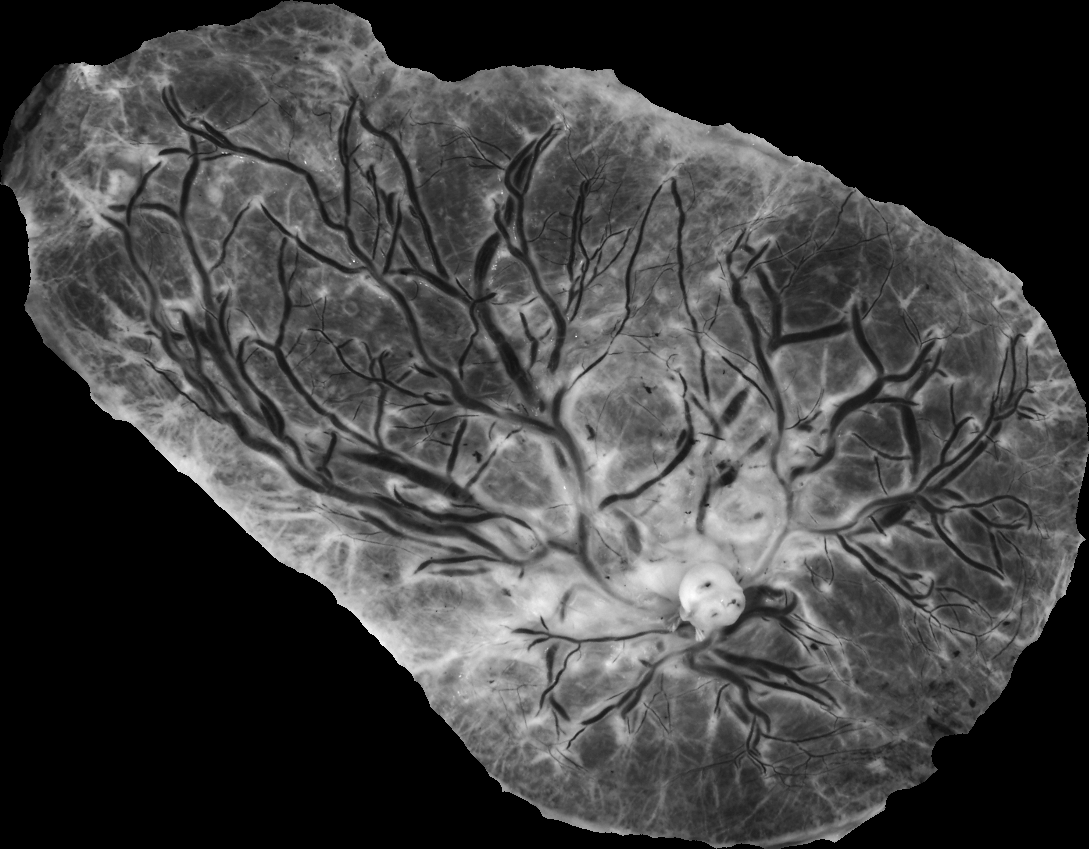
\includegraphics[width=0.48\linewidth]{qthresh_demo_img}}
\subfloat{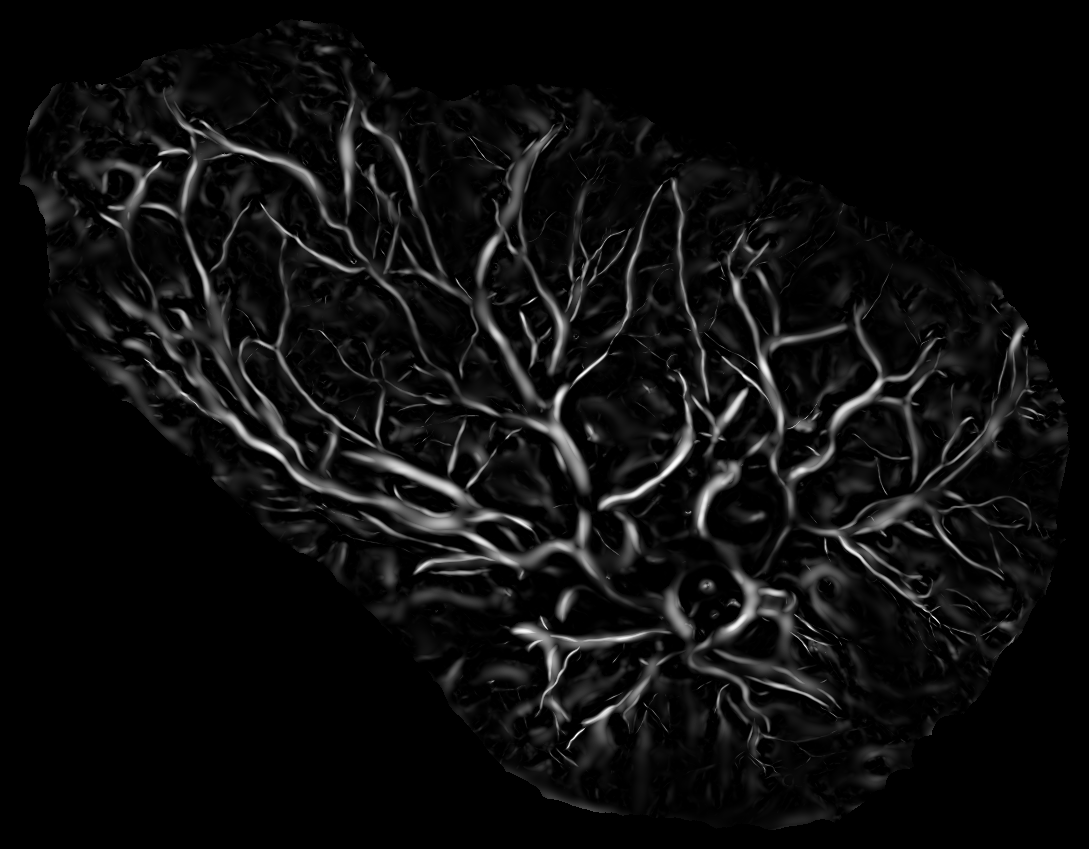
\includegraphics[width=0.48\linewidth]{qthresh_demo_Fmax}} \\
\subfloat{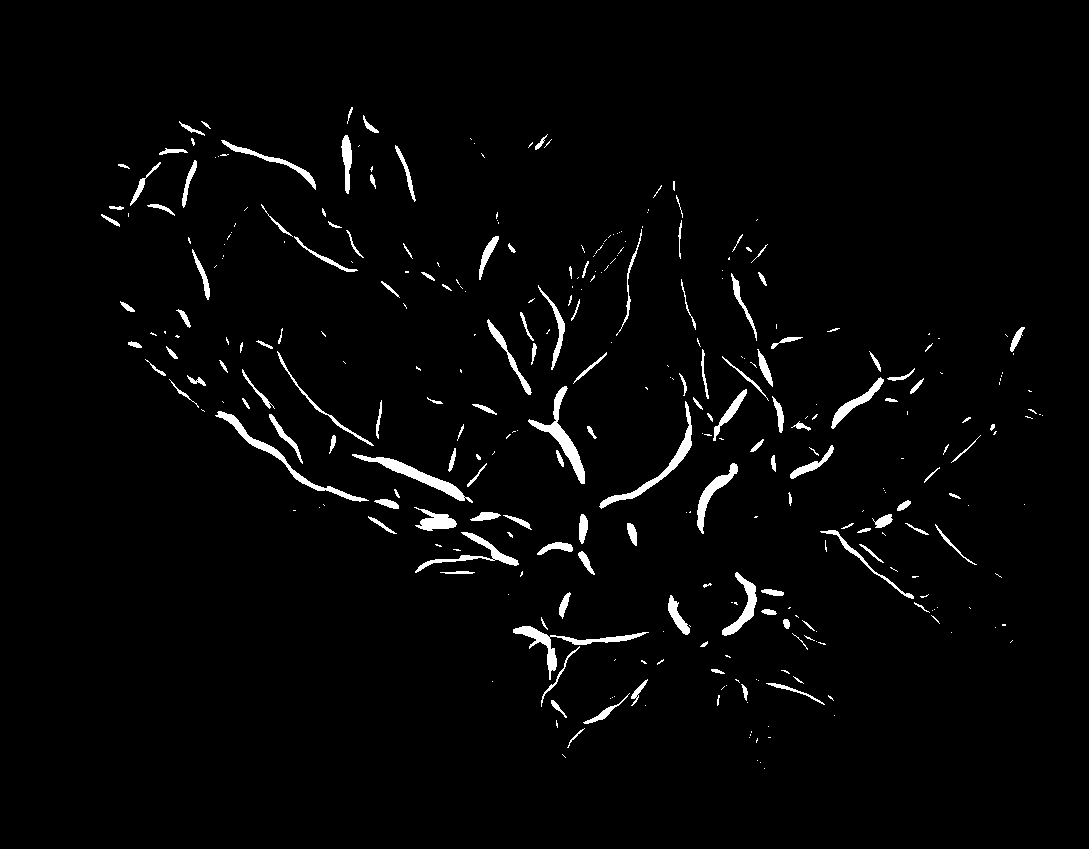
\includegraphics[width=0.48\linewidth]{qthresh_demo_q95}}
\subfloat{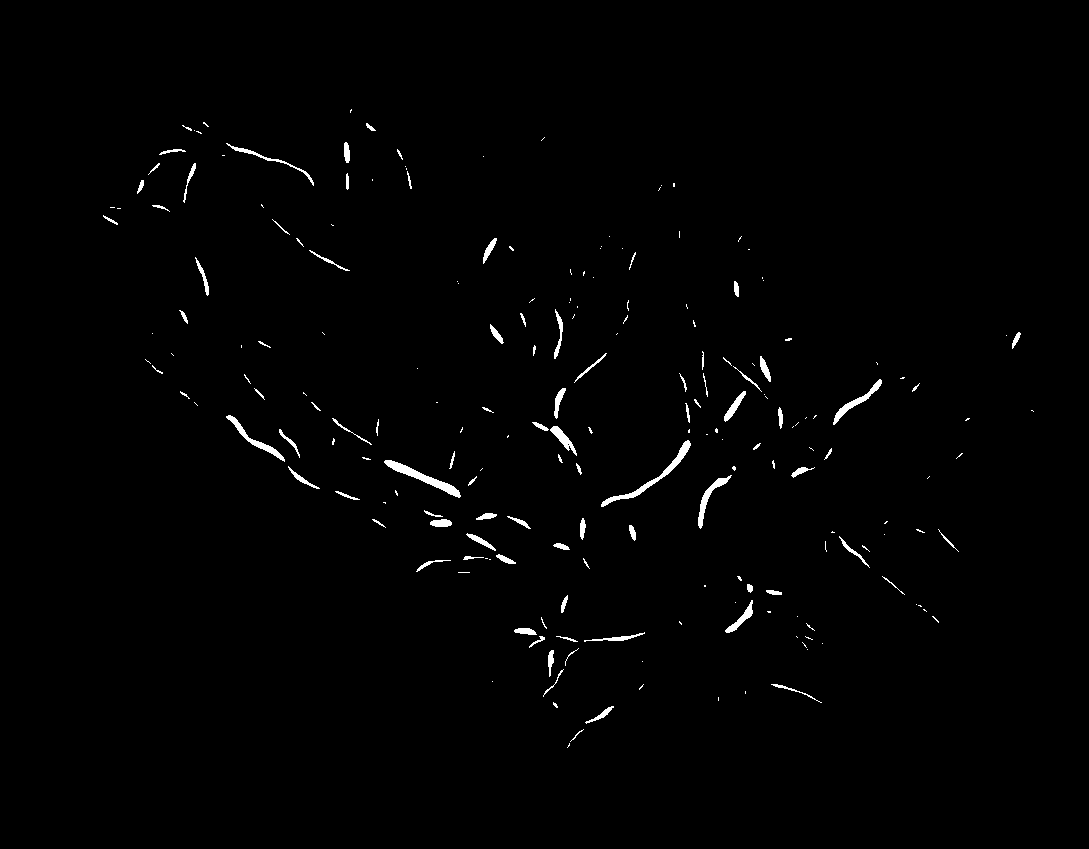
\includegraphics[width=0.48\linewidth]{qthresh_demo_q98}} \\
\caption{Nonzero-percentile thresholding of \Vmax (95th and 98th percentile)}.
\label{fig:qthresh_demo}
\end{figure}

Of course, the downside of this method is that we do not know in general the size of the network, and  we may miss entire branches of the vascular network if there is a large amount of curvilinear content elsewhere in the image.

We will discuss alternatives methods of aggregating results from our multiscale method, as well as optimal values for parameters and scales
in \cref{ch:segmentation}. As a final note, we admit that any future extensions of this work (as will be discussed in \cref{ch:conclusion}) need not proceed from either of these thresholdings; analyzing the raw vesselness score \Vmax, or even the un-merged scale-wise scores may prove far more rewarding.

\section{The Signed Frangi Filter} \label{sec:signed-frangi-filter}
We finally introduce the novel (yet straightforward) notion of the signed Frangi filter. As will be shown in \cref{ch:segmentation}, we can befefit from simultaneously calculate for a dark background and a light background. Since the Frangi filter normally throws away any response where $\lambda_2 < 0$ (if dark curvilinear features are targeted) or $\lambda_2 >0$ (if light curvilinear features are targeted), we lose no computation time at all (although we must store more results). After computing the multiscale result, we can easily separate these into a positive and a negative strain, which we will denote
$\Vmax^{(+)}$ and $\Vmax^{(-)}$. Our $\Vmax^{(+)}$ is the same as our $\Vmax$ before, and $\Vmax^{(-)}$ is the same result as if we had taken the Frangi filter while only looking for the opposite type (light/dark) curvilinear feature. Plotting $\Vmax$ over a scale of $[-1,1]$ demonstrates an interesting effect, as shown in \cref{fig:signsweep-2}. Whereas the Frangi filter generally is not reliable in terms of accurately predicting widths of trough-like (or ridge-like) curvilinear features, by somehow combining the results of our positive and negative strains. We \textit{can} get a sense of the width by looking at where there is a relatively strong response of opposite sign. We will develop a method of utilizing this observation in \cref{ch:segmentation}.


All that remains to describe mathematically is how to actually calculate the derivatives of our images and deal with the ultimately discrete nature of our samples.    